%%%%%%%%%%%%%%%%%%%%%%% file template.tex %%%%%%%%%%%%%%%%%%%%%%%%%
%
% This is a template file for Web of Conferences Journal
%
% Copy it to a new file with a new name and use it as the basis
% for your article
%
%%%%%%%%%%%%%%%%%%%%%%%%%% EDP Science %%%%%%%%%%%%%%%%%%%%%%%%%%%%
%
%%%\documentclass[option]{webofc}
%%% "twocolumn" for typesetting an article in two columns format (default one column)
%
\documentclass{webofc}
\usepackage[varg]{txfonts}   % Web of Conferences font
\usepackage{hyperref}
\usepackage{natbib}
\usepackage{caption}
\usepackage{subcaption}
%
% Put here some packages required or/and some personnal commands
%
%
\begin{document}
%
\title{Improving GlideinWMS factory site configuration with automation tools}
%
% subtitle is optionnal
%
%%%\subtitle{Do you have a subtitle?\\ If so, write it here}

\author{\firstname{First author} \lastname{First author}\inst{1,3}\fnsep\thanks{\email{Mail address for first
    author}} \and
        \firstname{Second author} \lastname{Second author}\inst{2}\fnsep\thanks{\email{Mail address for second
             author if necessary}} \and
        \firstname{Third author} \lastname{Third author}\inst{3}\fnsep\thanks{\email{Mail address for last
             author if necessary}}
        % etc.
}

\institute{Insert the first address here 
\and
           the second here 
\and
           Last address
          }

\abstract{%
  Insert your english abstract here.
}
%
\maketitle
%
\section{Introduction}
\label{intro}
The Open Science Grid (OSG) \cite{OSG} is a consortium of universities and federal labs that contribute compute resources for scientific research across multiple domains. Members consist of the providers of the resources and the researchers who consume them. Each resource provider has their own collection of machines which are usually made accessible to users with a scheduling system commonly referred to as a batch system, such as HTCondor \cite{HTCondorURL} or Slurm \cite{SlurmURL}. %TODO PBS, SGe. Others?
These systems sufficiently meet the needs of local users who have local accounts at specific institutions, however typically a scientific collaboration may own or have access to hardware across multiple institutions. Meta-scheduling systems have been developed to facilitate this use case. One popular meta-scheduling system type commonly used in Grid Computing is known as the pilot system \cite{GlideinWMS}. A pilot system sends placeholder jobs into the various local batch systems at multiple institutions. Once the pilot jobs start up, it retains a claim on a physical resource for some agreed on amount of time.
Then, they typically connect back to a central database belonging to the meta-scheduler and they advertise the available resource. Then, the meta-scheduler assigns real user jobs to the resources claimed by the pilots. 

The OSG has adapted GlideinWMS \cite{GlideinWMSURL} as the primary pilot system to support meta-scheduling across its resources. Sites that want to expose resources to OSG to accept compute jobs, also require additional software known as a Compute Entrypoint (CE), which acts as a doorway into the batch system. It is responsible for authenticating the incoming pilots, mapping them to a particular user account, and routing them to the appropriate resources for the respective community they represent. The OSG provides the HTCondor-CE \cite{}, %TODO add reference
either in the form of software packages for sites to install and maintain their own, or as a service known as a Hosted CE \cite{}, %TODO reference
which is one OSG Operations staff spins up and operates on behalf of a site.

Pilot jobs are submitted to CEs by a central GlideinWMS service, called  factory. The maintenance of the CE configurations in the factory is a challenging task done by a small set of operators that interact with CE administrators. In this paper we discuss how the configuration management of the OSG factory has improved with the development and usage of automation tools.

% need section here to move detail from intro.. 
\section{Motivation}

\subsection{Accessing CEs using GlideinWMS}

% somewhere in Motivation, cite previous CRIC work

Depending on the job workflow, particular resources of certain types and sizes may be required and need to be specified. For example, a job may be single core and require a minimum of two gigabytes, or it may be a multicore job, and require 16 cores and 64 gigabytes of ram. Other jobs might require special nodes that have enabled GPU support. In order to handle these cases, the GlideinWMS meta-scheduler must be able to request pilots with the corresponding attributes reflecting the user job requirements. These attributes then get passed to the site CE during the pilot submission time. It is the responsibility of the CE administrator to ensure the attributes of the incoming pilots can map to particular resources in the batch system, and the HTCondor-CE provides job routing configuration to handle this.

In addition to the factory, the other main component of GlideinWMS is called the frontend. The factory and frontend are independent services that are typically run on different hardware and are maintained by different people. Each scientific community, also known as Virtual Organization (VO), typically has its own frontend. This component is responsible for tracking user job requests, and translates them to pilot submission requests. The factory is the central component that is responsible for receiving frontend requests, and performs the actual pilot submissions. There is one central OSG Glidein Factory that serves all of the VO frontends that are registered to it, and is run by the Factory Operations team. In order for the frontend to request appropriate resources on the grid to support particular user jobs, it needs to know the available pilot sizes at all of the possible compute sites. %TODO Feels like the sentence is a bit cumbersome
Compute resources between sites, and even within a single site, are in general heterogeneous. Machines can have any number of total cores, memory, and may or may not have GPUs. Different sites may have different policies concerning which VOs they allow to enter their CE, as well as which resources are available to a particular VO. Other policies may specify the maximum number of pilots for a particular VO that are allowed to run at any given time, and how much time pilots are allowed to claim the resources.

All of the known possible pilot configurations for all sites that the frontend needs to be aware of in its decision making are contained in the factory configuration. A particular configuration for a particular pilot in the factory is known as an entry. The entry contains fields that include information about how to submit to the the CE, such as its hostname and port, the required CE attributes to obtain the correct resources at that particular site, and all of the attributes describing the size and policies for this pilot type. One major task for the Factory Operations team is maintaining the set of entries. As new resources are made available to VOs, new entries must be created. As resources are updated and site policies change, the entries may need to be updated to reflect those changes. Significant effort is required to keep the entry configurations up to date, and it often requires direct input from site administrators via service ticket exchanges. The Factory Operations team has been working to reduce the human effort required in the entry configuration upkeep. This has resulted in the development of new software tools which have become a part of the GlideinWMS codebase, and are used to automatically generate factory entry configurations. The goal of these new automation tools is to streamline the process in how entries are created, and give more control to site administrators so that they can directly update entries of pilots submitted to their sites while depending less on long communication chains with the Factory Operations team.


\section{Architecture}
\label{arch}
The GlideinWMS Factory entry automation tools leverage information systems that describe site resources on the grid. The OSG has an existing system called the OSG CE Collector. The CE Collector consists of a HTCondor collector daemon which acts as a simple key-value data store. Each HTCondor CE that is installed from the standard OSG software repository packages contains a tool called OSG-Configure which can be used to publish descriptions of resources accessible from the corresponding CE. The CE can be queried manually using the standard HTCondor client tool, \verb"condor_status", or using the HTCondor Python bindings library \cite{}. %TODO add reference

A script called \verb"OSG_autoconf" was developed by the Factory Operations team. It is run by a Factory operator from the command line to synchronize the factory entry configurations with the CE Collector database. Before final synchronization, there is an intermediate merge step that takes place. Currently, a complete factory entry cannot be created from the information only coming from the CE Collector. It only contains a subset of fields that can be used as a starting point. Also, factory operators need the ability to override the fields that do come in from the Collector, because they are not guaranteed to be correct. To handle this, the \verb"OSG_autoconf" script also parses a configurable set of YAML files known as whitelist files. In addition to providing operators the ability to arbitrarily override incoming fields from the collector and add additional fields, the operators can decide which advertised CEs they would like to propagate from the CE Collector to the factory entries. This ability is fundamental because not all advertised CEs are necessarily operational or production ready, or even are configured accept pilots from the GlideinWMS system.

One design challenge encountered is that the OSG CE Collector does not have persistent state. If a CE is temporarily malfunctioning, it will stop advertising itself, and after a period of time the ad describing it will disappear from the Collector. To handle this, \verb"OSG_autoconf" always caches the entire results of the CE Collector query to disk in a file called \verb"OSG.yml" on each run. Before the merge step, the script compares the whitelist files to the new query results, and if a CE is in the whitelist files but is no longer found, it will attempt to recreate the entry by merging with the cached results from \verb"OSG.yml" of the previous attempt. It also stores the previous cached query result into another file, \verb"missing.yml" before updating \verb"OSG.yml" so that it can continue to recreate the entry on subsequent runs, until the CE propagates back to the CE Collector.

\begin{figure}
    \centering
    \begin{subfigure}[b]{\textwidth}
        \centering
        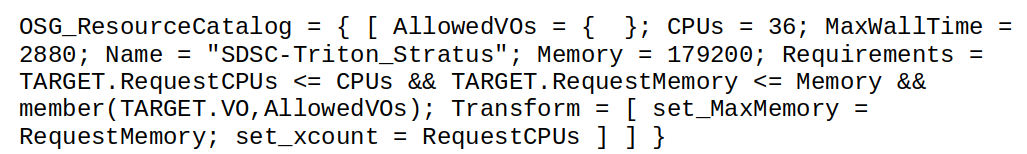
\includegraphics[width=\textwidth]{images/triton_collector.png}
        \caption{CE Collector output}
        \label{fig:ce_col}
    \end{subfigure}
    \begin{subfigure}[b]{0.4\textwidth}
        \centering
        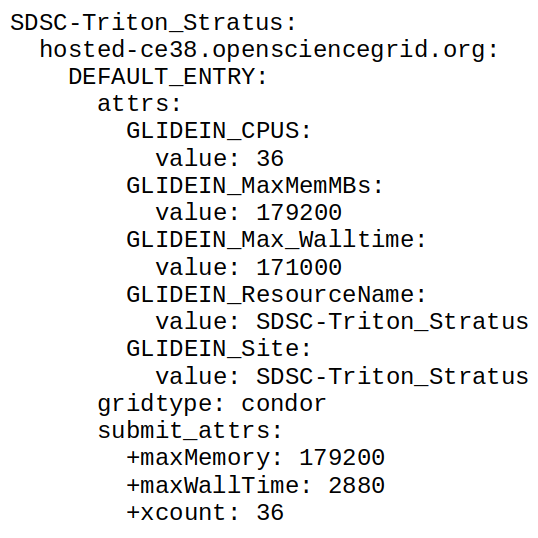
\includegraphics[width=\textwidth]{images/triton_osg_yml.png}
        \caption{OSG.yml}
        \label{fig:osg_yml}
    \end{subfigure}
    \begin{subfigure}[b]{0.4\textwidth}
        \centering
        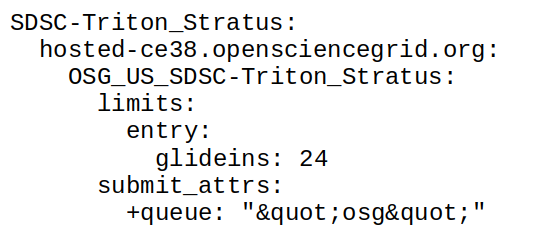
\includegraphics[width=\textwidth]{images/triton_whitelist.png}
        \caption{whitelist.yml}
        \label{fig:whitelist_yml}
    \end{subfigure}
    \begin{subfigure}[b]{\textwidth}
        \centering
        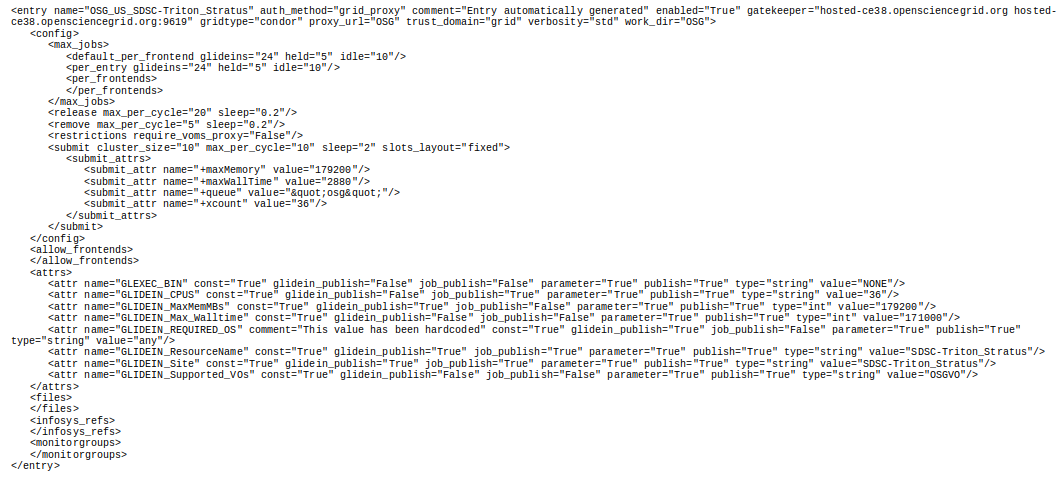
\includegraphics[width=\textwidth]{images/triton_entry.png}
        \caption{generated entry}
        \label{fig:entry}
    \end{subfigure}
    \caption{The auto-generation script reads values in for a particular CE from the Collector as shown in Figure \ref{fig:ce_col}. It processes the fields into a format the factory expects, merges with default values, and stores it on disk in OSG.yml as seen in Figure \ref{fig:osg_yml}. Next, it gets selected by the example whitelist.yml file in Figure \ref{fig:whitelist_yml}, picks up any overrides, and merges the data to generate the entry as shown in Figure \ref{fig:entry}} 
    \label{fig:arch}
\end{figure}

\section{Operational experience}
\label{exp}
To test the automatic entry generation proof of concept, the Factory Operations team decided to limit the scope of sites to those served by the OSG Hosted CE. The advantage of testing auto-generation on Hosted CEs is that Factory Operators work more closely with the central OSG Operators responsible for administering them. If changes need to be applied on the CE, there is much quicker turnaround time. Also Hosted CE operators have direct access to the Factory configuration, and can directly create and make changes to entries serving their CEs without needing to request a change from the Factory Operations team.

The factory currently has 28 entries describing Hosted CEs under auto-generation, across 20 unique sites. Over the course of maintaining a variety of configurations, patterns have emerged suggesting limitations in the ability for CE administrators to advertise pilot configurations with the OSG-Configure tool. Traditionally, the section that gets published to the OSG Collector was intended to advertise specific machine types in their cluster. As an example, suppose a hypothetical site has a CE pointing to different generations of hardware. Some machines have eight cores and 24 gigabytes of memory, some have eight cores and 16 gigabytes of memory, and some have four cores and 16 gigabytes of memory. To completely expose all of these combinations in GlideinWMS, the factory would require four entries to describe the resources behind this CE. Now suppose on average a site has O(10) types. The current factory configuration has O(100) CEs total. This would require there to be O(1000) entries to describe all the resources on the grid. There is currently 566 actual entries total in the production factory. Growing the number of entries by an order of magnitude not only would have unknown scaling consequences in the system, it would be much harder to maintain.

The solution to this is to instead configure the best fit pilot for a given site. Consider the hypothetical site above. A single entry describing a pilot with four cores and four gigabytes of memory would fill all of the cores without fragmentation, but with some memory left unclaimed in some cases. This is an acceptable compromise, and at base level it reduces the total required entries by an order of magnitude. The \verb"OSG_autoconf" tool has rules to calculate the best fit pilot in the case where a CE configuration advertises many machine sizes. In the case of Hosted CEs, the Factory Operations team has shown the Hosted CE operators how to declare pilot sizes rather than machine type sizes, to better streamline the configuration of the entries. However longer term the Factory Operations team is working with the OSG Software team to provide site administrators a way to communicate from OSG-Configure that they are advertising their preferred pilot size rather than machine size. That way, there will be no ambiguity in how to configure the pilots.

% (room for improvement - push more fields not currently supported by osg_configure in so they do not haveto be put in as overrides, gpu support -> future plans)

\section{Future plans}
\label{future}
While the OSG Software team is working on the addition of the pilot section in the OSG-Configure tool, the Factory Operation team has been updating the auto-generation tools to accept the new sections of CE configuration. Care must be taken to ensure that the merge step still works if this optional setting is not used, to remain backward compatibility. The current hierarchy in the whitelist file YAML tree is structured has levels for Site and CE, followed by a list of entry names to be generated from a particular Site-CE combination. Multiple entries can be derived from a single CE configuration by listing multiple entry names, and overriding variables accordingly. The current solution under investigation to incorporate published pilot configurations under a particular CE is to extend the YAML hierarchy to include a new pilot level under the CE level. Then, whitelisted entry names can use a particular pilot level as a starting point. For CEs that do not advertise any pilot sections, a default pilot level with the special keyword name \verb"BEST_FIT" is given, to signify the configuration falls back to providing a single best fit pilot to be used as a starting point. Some basic one time file edits will be required to put the new \verb"BEST_FIT" level into existing whitelist files in production that do not yet contain it, but once it is added, the auto-generation tools will continue to work as expected.

\begin{figure}[h]
\centering
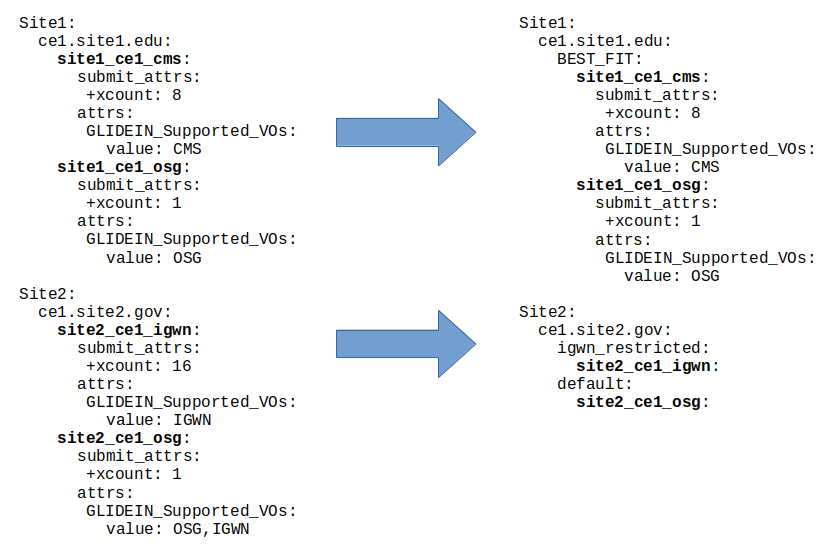
\includegraphics[width=\textwidth]{images/autoconf_new_layer.png}
\caption{Old whitelist example vs new with additional pilot layer, creating two entries for two sites. Site2 provides its own pilot sections, so field overrides describing allowed VOs and core counts are no longer needed in the whitelist}
\label{fig:newlayer}
\end{figure}

% add some lines about incorporating CEs beyond hosted CEs, revisiting CRIC as an additional data source for WLCG sites, more automation / cron, etc? (have not mentioned receiving updates when sites change their configurations)
% highlight the end goal is simplify the whitelist as much as possible, ideal is for fatory operators to just list, only override values where absoluely necessary. giving site admins more control by exposing pilot configurations

\section{Conclusions}
\label{conclusions}
Factory entry auto-generation tools were created to reduce the burden of one of the most time consuming aspects of Factory Operations --- the task of keeping up with site changes. By leveraging existing information systems such as the OSG CE Collector, Factory operators are able to give back some control directly to the site administrators, who know the topology of their resources best. By carefully describing their resources in the form of pilot descriptions, site administrators can directly ensure claims on their resources are being optimized. For example, they can make changes immediately to their CE configurations whenever they add new physical machines, or decommission old ones, without having to open a chain of communication to Factory operations. They can add new pilot sections to describe special restricted resources such as GPUs, or nodes for which they only want specific experiments to have access. In this case the only responsibility of the site administrator is to notify Factory Operations when they are ready for this new pilot type to be whitelisted. The details of the configuration itself will be sent over through the information system. By using automation to streamline the process of factory entry upkeep, overall quality of service will increase for GlideinWMS based pilot systems because Factory Operators can spend less time configuring entries and more time assisting administrators in debugging equally important things such as why pilots might be failing at a site, or why a site is not optimizing its resources. These activities will always be a vital part of routine factory operations in ensuring quality of service on the Grid.


% BibTeX or Biber users please use (the style is already called in the class, ensure that the "woc.bst" style is in your local directory)
\bibliography{papers}
%
% Non-BibTeX users please use
%
%\begin{thebibliography}{}
%
% and use \bibitem to create references.
%
%\bibitem{RefJ}
% Format for Journal Reference
%Journal Author, Journal \textbf{Volume}, page numbers (year)
% Format for books
%\bibitem{RefB}
%Book Author, \textit{Book title} (Publisher, place, year) page numbers
% etc
%\end{thebibliography}

\end{document}

% end of file template.tex